\section{Intro}\label{sec:intro}
Over the last two decades Machine Learning (ML) algorithms have advanced drastically to the extent that they are portable
enough to be carried in our pockets or to be executed on a device with similar hardware constraints such as a \textit{RaspberryPi} microcomputer.\\
Due to increasing amount of interest in the development of faster and computationally better GPUs, in combination with the
growing amount of available data, Deep Learning (DL), a field of Machine Learning, started to gain popularity. The
groundbreaking 1998 paper by Yann LeCun et al.~\cite{Lecun99objectrecognition} introduced \textit{LeNet-5}, a Convolutional Neural Network (CNN)
architecture, designed for recognition of handwritten check numbers.\\
More than a decade later the \textit{AlexNet} model ~\cite{AlexNet} won the 2012 ImageNet ILSVRC challenge by a large margin.
\textit{AlexNet} is structured similarly to \textit{LeNet-5}, but has much more parameters, which gave it the advantage over other submissions in that year.
Hence, \textit{AlexNet} is considered to mark the start of widely spread Deep CNNs in research and industry.\\
Since then many new CNN architectures got introduced that reached even higher scores in similar competitions, such as
the \text{VGG-16} ~\cite{VGG16} or \textit{MobileNet} ~\cite{MobileNet} models, which will be used here for benchmark comparisons.
Deep NNs and Deep CNNs are not limited to solve computer vision tasks, they can be used to solve a wide variety of
problems, e.g. solving tasks like speech recognition using audio data, analyzing trends in the stock marked based on tabular data or predicting sentences for emails using textual data.\newline
The following section will describe the motivation behind this paper, give an introduction into the problems that are being solved, briefly review existing work in the field and give an overview about the following sections.

\subsection{Motivation}\label{subsec:motivation}

\begin{figure}[!ht]
    \centering
    \begin{minipage}[t]{.4\textwidth}
        \vspace{0pt}
        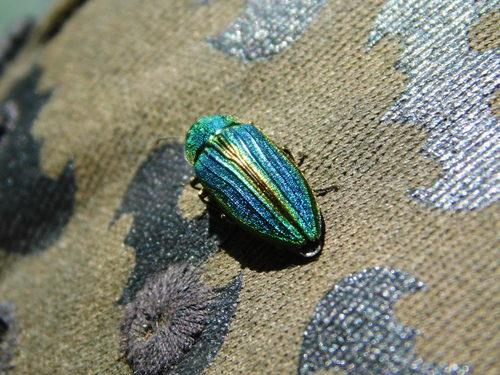
\includegraphics[width=\textwidth]{images/00185_Coleoptera_Buprestidae_0a92c2b4-ca55-4f52-850b-3718920d2c9f.jpg}
        \caption{Coleoptera sample}
        \label{fig:coleoptera-sample}
    \end{minipage}
    \hfill
    \begin{minipage}[t]{.4\textwidth}
        \vspace{0pt}
        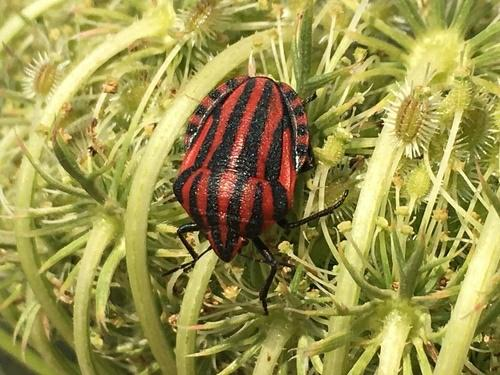
\includegraphics[width=\textwidth]{images/00624_Hemiptera_Pentatomidae_5ee497cb-1230-4743-b455-49e77bad4eb9.jpg}
        \caption{Hemiptera sample}
        \label{fig:hemiptera-sample}
    \end{minipage}
    \begin{minipage}[t]{.4\textwidth}
        \vspace{0.3cm}
        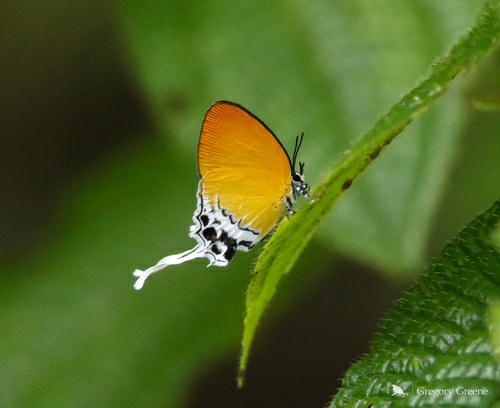
\includegraphics[width=\textwidth]{images/01471_Lepidoptera_Lycaenidae_6ba490d2-8d07-4d44-97b3-b8f1fc48b5b5.jpg}
        \caption{Lepidoptera sample}
        \label{fig:lepidoptera-sample}
    \end{minipage}
    \hfill
    \begin{minipage}[t]{.4\textwidth}
        \vspace{0.3cm}
        \includegraphics[width=\textwidth]{images/02312_Odonata_Aeshnidae_1aefce10-69b6-456a-88ad-ae1d3a11b2e6.jpg}
        \caption{Odonata sample}
        \label{fig:odonata-sample}
    \end{minipage}
    \begin{minipage}[t]{.4\textwidth}
        \vspace{0.3cm}
        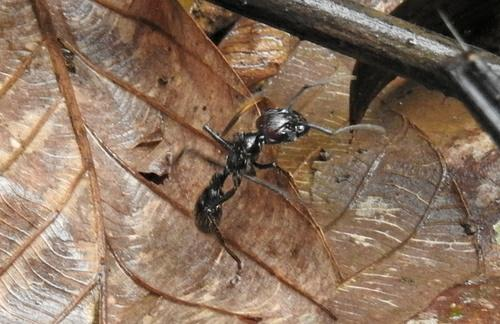
\includegraphics[width=\textwidth]{images/00761_Hymenoptera_Formicidae_eaf1dd96-d5bb-44c2-96b3-220c8104598d.jpg}
        \caption{Hymenoptera sample}
        \label{fig:hymenoptera-sample}
    \end{minipage}
\end{figure}

The 2017 paper of Caspar A. Hallman et al.~\cite{biomassPaper} revealed shocking facts about the reduction of biomass over the last decades.\\
The authors explain that their results of 27 years of research, in lowland areas of west Germany, give them reason to estimate a seasonal decline of 76\%, and midsummer decline of 82\% in flying insect biomass.
Additionally, the researchers point out that this decline is not dependent on the habitat type, however a change in weather or habitat can not explain this overall decline.
Furthermore, the paper states that this decline is evident throughout growing season and irrespective of habitat type or landscape configuration, which suggests the involvement of large-scale factors.
Unfortunately the researchers were not able to incorporate factors such as pesticide usage, increased usage of fertilizers or frequency of agronomic measures, which may form a plausible cause.\\
To make people aware of this problem and of insects' role in the environment as well as to start the process of collecting more insights, about this decline in biomass, the \href{https://kinsecta.org}{\textit{KInsecta}}~\footnote{KInsecta project website: \url{https://kinsecta.org/}} project  was formed.
\textit{KInsecta} is a citizen science project
~\footnote{Citizen Scientist: a member of the general public who collects and analyses data relating to the natural world, typically as part of a collaborative project with professional scientists.}
of BHT in cooperation with the \href{http://listhof-reutlingen.de/}{UBZ Listhof}~\footnote{UBZ Listhof website: \url{https://listhof-reutlingen.de/}} and is part of the funding programm "KI-Leuttürme für Umwelt, Klima, Natur und Ressourcen".
Its objective is to build a device capable of monitoring insects in a local area, e.g. a garden.
The device works in a way that, in contrast to other monitoring techniques, collects data about insects in the area where it is deployed without harming the individual.
Instead of killing or collecting insects alive for later analysis, \textit{KInsecta}'s monitoring device uses different sensors, such as a
\textit{Wingbeat}~\footnote{
The \textit{Wingbeat} sensor is an effort of the \textit{KInsecta} project team, a reference page can be found at \url{https://kinsecta.org/sensorik-2\#wingbeat} (German).
}
sensor to detect wing beat frequencies, and a high resolution camera to collect visual data.
The camera module and an experimental setup can be seen in \figref{fig:camera}, \figref{fig:camera-look-through} and  \figref{fig:experiment-setup}.\\
The collected data of the \textit{Wingbeat} sensor will eventually get processed by a custom ML classifier.
In addition to that, the device misses a computer vision classifier to process the images collected from the camera.
This thesis investigates different ML methods to set the ground to build an extendable, stable algorithm to detect insects in images.

Detecting and classifying objects in images is not a novel task, solutions to this task have been around for decades.
But most techniques require a lot of pre-processing work on the input data, different methods to apply to the images and/or a lot of computational resources such as RAM.
Where conventional approaches are too dependent on one task, existing ML Models seem to be too complex and too resource intense. Hence a tailored architecture is desired.

\subsection{Problem description}\label{subsec:problem-description}
As the title suggests this thesis focuses on different methods to localize and classify insects in image data.
The tasks of localization and classification can be solved in different ways using different techniques.
The main question this paper will try to answer is, if there is a ML method which solves both tasks in an acceptable manner, while following resource and architecture constraints to allow usage of the resulting program on a \textit{Raspberry Pi}.\\
The acceptance criteria for such method is called a metric, that is either, in the case of the classification task, the accuracy of correct predictions, or in case of localization, further also called Bounding Box regression (BBReg), a visual comparison of predicted Bounding Boxes (BBs) with their corresponding ground truth, the \hyperref[eq:giou]{\textit{GIoU}} metric. The exact definition of these metrics can be found in the subsection "\nameref{subsec:metrics}".\\
Generally speaking the objective of this thesis is to use image data, such as the example images
\figref{fig:coleoptera-sample}, \figref{fig:hemiptera-sample}, \figref{fig:lepidoptera-sample}, \figref{fig:odonata-sample} and \figref{fig:hymenoptera-sample}
~\footnote{Image Credits:
\ref{fig:coleoptera-sample} (CC-BY-NC) by user "m3d5" \url{https://www.inaturalist.org/observations/36275496},
\ref{fig:hemiptera-sample} (CC-BY-NC) Observation © Uriah Resheff  \url{https://www.inaturalist.org/observations/13067479},
\ref{fig:lepidoptera-sample}(CC-BY-NC) Observation © Gregory Greene \url{https://www.inaturalist.org/observations/30220853},
\ref{fig:odonata-sample} (CC-BY-NC) Observation © orewoet \url{https://www.inaturalist.org/observations/32606254} and
\ref{fig:hymenoptera-sample} (CC-0) Observation © Wouter Koch}
, process them using a ML method to then obtain a class label with an
accuracy comparable to results presented in the 2017 iNat data set paper~\cite{iNat}.
To do so, two approaches are chosen.\\
First, in the \textbf{two-stage-method}, two dedicated methods process the input data to come to a final conclusion of a class label, as displayed in \figref{fig:independent-method}.
One method is used to first detect insects in the raw input images, by predicting BB coordinates.
After obtaining the coordinates the input image gets cropped to then only contain the patch covered in the BB.
The resulting cropped image will then be used as input image for another method that will perform the classification task on it to obtain a class label.\\
For the \textbf{single-stage-method}, methods get explored that can solve both tasks at the same time, either in parallel or by building onto each other as displayed in \figref{fig:joint-method}.

\begin{figure}[!ht]
    \begin{minipage}{.45\textwidth}
    \centering
    \begin{tikzpicture}
    \SetEdgeStyle[TextFillOpacity=0]

    \node (input) at (0, 8) {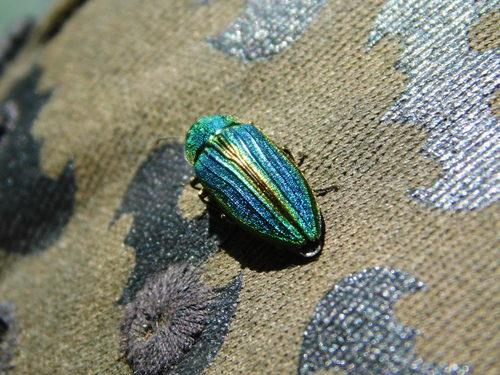
\includegraphics[width=.6\textwidth]{images/00185_Coleoptera_Buprestidae_0a92c2b4-ca55-4f52-850b-3718920d2c9f.jpg}};
    \node (bb) at (0, 4) {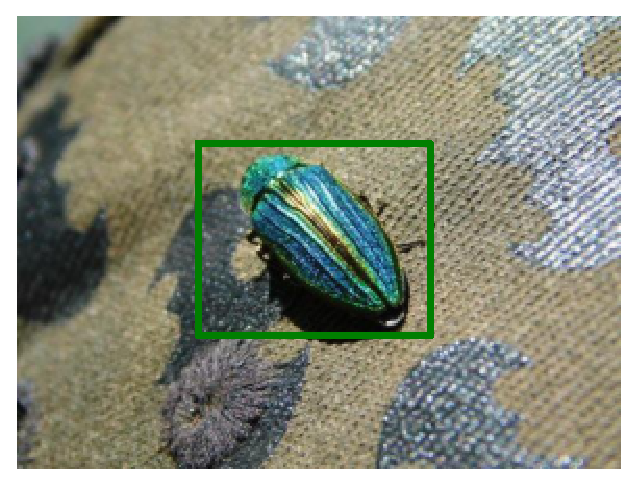
\includegraphics[width=.6\textwidth]{images/perfect-prediction-without-label.eps}};
    %\node (c) at (0, 0) {\includegraphics[width=.125\textwidth]{images/cropped-00185_Coleoptera_Buprestidae_0a92c2b4-ca55-4f52-850b-3718920d2c9f.jpg}};
    %\node[text width=1.5cm] (model2) at (2, 2){Clas\-si\-fi\-ca\-tion};
    \node (label) at (0, 0) {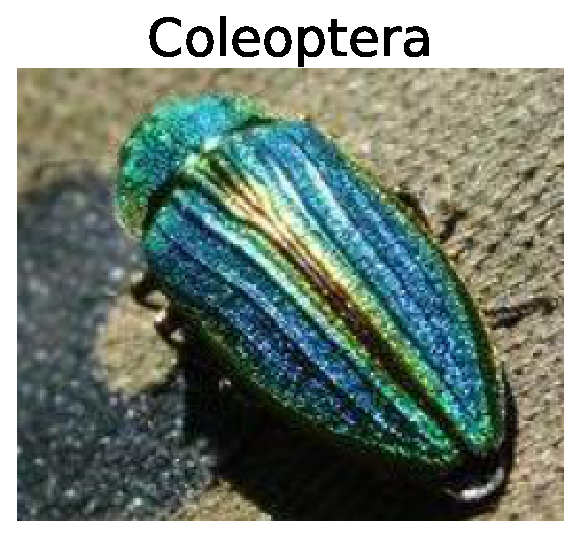
\includegraphics[width=.6\textwidth]{images/cropped-00185_coleoptera.eps}};

    \Edge[Direct,label=Localization,position=right](input.south)(bb.north)
    \Edge[Direct,label=Classification,position=right](bb.south)(label.north)


    \end{tikzpicture}

    \caption{\textbf{2-stage-method}, top down: an image gets passed to a method solving the localization task, then the input image gets cropped to the shape of the predicted BB. At the end a second method is used to obtain the class label.}
    \label{fig:independent-method}
    \end{minipage}
    \hfill
    \begin{minipage}{.45\textwidth}

    \vspace{2.8cm}
        \centering
        \begin{tikzpicture}
        \SetEdgeStyle[TextFillOpacity=0]

        \node (input) at (0, 4) {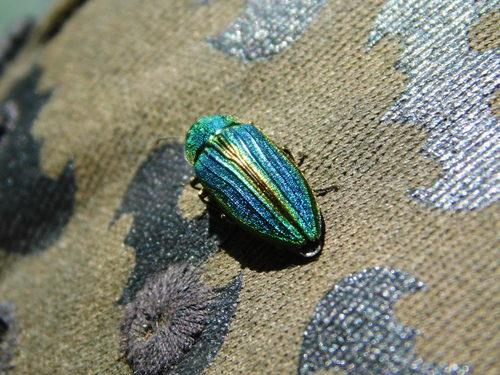
\includegraphics[width=.6\textwidth]{images/00185_Coleoptera_Buprestidae_0a92c2b4-ca55-4f52-850b-3718920d2c9f.jpg}};
        \node (bb) at (0, 0) {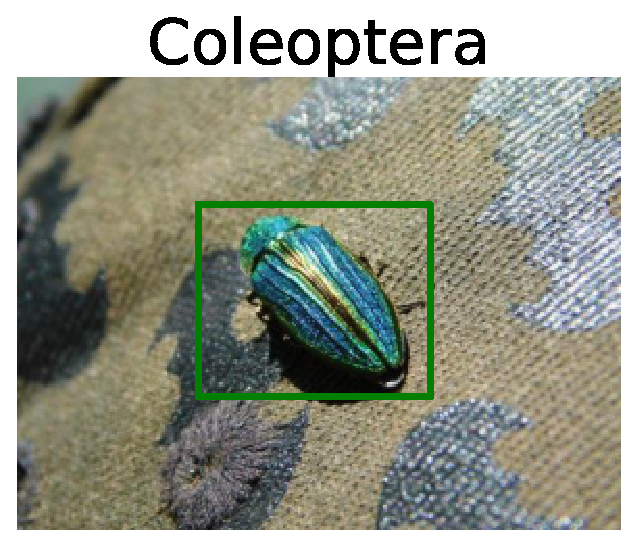
\includegraphics[width=.6\textwidth]{images/perfect-prediction.eps}};

        \Edge[Direct,label=Detection,position=right](input.south)(bb.north)


        \end{tikzpicture}

        \caption{\textbf{Single-stage-method}, an image gets processed by a method that outputs a Bounding Box and a classification label prediction.}
        \label{fig:joint-method}

    \end{minipage}
\end{figure}


\subsection{Existing work in the field}\label{subsec:existing-work-in-the-field}
As stated in the introduction, since the publication of \textit{AlexNet} a wide range of new computer vision, specifically object detection, architectures got released, including \textit{VGG-16} and \textit{MobileNet}.
Both of these architectures were designed with the objective of solving a classification task and generally output extracted features from the input images to either predict one out of 1000 (VGG-16) or 200 (MobileNet) classes.
Hence, both can be grouped together with methods that solve the tasks individually, using two independent methods or in this case model instances.
In 2016 Redmon et al.~\cite{yolo} introduced a novel architecture, \textit{YOLO}, that contains a single Neural Network that predicts Bounding Boxes and class probabilities directly from full images in one evaluation, which is the reason for the name of this architecture, \textbf{Y}ou \textbf{O}nly \textbf{L}ook \textbf{O}nce.
YOLO essentially subdivides the image into regions and predicts BBs and probabilities for each region.
Another architecture is \textit{MobileNet-SSD} from the \textit{MobileNet}~\cite{MobileNet} paper. An architecture based on the \textbf{S}ingle \textbf{S}hot \textbf{D}etection framework~\cite{SSD}, that essentially works the same way as YOLO.
Both of these methods are part of the previously mentioned \textbf{single-stage-method} approach to solve the detection problem.
But most of these industry standard architectures come with a big disadvantage.
To generalize over a wide range of tasks and to generalize big fractions of the training set the models contain a huge number of parameters resulting in high resource requirements to train, maintain and use these models.\\
In the \nameref{sec:application} section we look deeper into problems of such architectures.
To make them available for devices like the \textit{RaspberryPi} a lightweight form can be created, e.g. by pruning the dense model into a sparse model or quantizing its floating point valued weights into integer values~\footnote{Some techniques are described e.g. in the \textit{Tensorflow} documentation \leavevmode\url{https://www.tensorflow.org/lite/performance/model_optimization}, in addition to that we will look closer into some of the techniques described there in a later section (\leavevmode\ref{subsec:hosting-on-raspberry}).}.
Each of these techniques will trade accuracy for size and computational speed.


\subsection{Approaches to solve the problem}\label{subsec:approaches-to-solve-the-problem}
There are many different solutions and approaches to both classification and regression tasks.
Using dedicated methods for each of the tasks, the 2-stage-method, or using a single method to solve both tasks at once, the single-stage-method, is one of the aspects this thesis analyzes.
After briefly reviewing conventional statistics methods such as \nameref{subsec:linear-regression}, or \nameref{subsec:support-vector-machines},
the reader is invited in the following sections to read more about modern methods such as \nameref{subsec:neural-networks} and \nameref{subsec:cnn} to solve both tasks individually or combined.
Whereas conventional methods allow fast solutions by precomputing required parameters, modern techniques require iterative algorithms to slowly adjust parameters until they converge to a solution.
This process of fitting parameters until they match a combination that results in satisfying outputs is called the training of an ML algorithm, also called training a model.
There are multiple ways of performing the training of a model, that will be discussed in \nameref{subsec:training-algorithms}.
Because the data set used here consists of pre-existing class labels, this work focuses on pure \textit{supervised learning} tasks.

\begin{wrapfigure}{r}{0.5\textwidth}
    \vspace{-0.5cm}
%\begin{figure}[!ht]
    \centering
    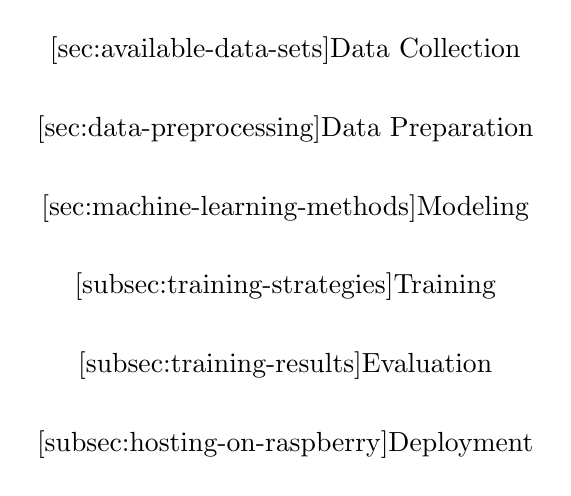
\begin{tikzpicture}
        \node[shape=rectangle] at (0, 5) (data){\leavevmode\hyperref[sec:available-data-sets]{Data Collection}};
        \node[shape=rectangle] at (0,  4) (cleaning){\leavevmode\hyperref[sec:data-preprocessing]{Data Preparation}};
        \node[shape=rectangle] at (0,  3) (modeling){\leavevmode\hyperref[sec:machine-learning-methods]{Modeling}};
        \node[shape=rectangle] at (0,  2) (training){\leavevmode\hyperref[subsec:training-strategies]{Training}};
        \node[shape=rectangle] at (0,  1) (evaluate){\leavevmode\hyperref[subsec:training-results]{Evaluation}};
        \node[shape=rectangle] at (0,  0) (deployment){\leavevmode\hyperref[subsec:hosting-on-raspberry]{Deployment}};

        \Edge[Direct](data)(cleaning)
        \Edge[Direct](cleaning)(modeling)
        \Edge[Direct](modeling)(training)
        \Edge[Direct](training)(evaluate)
        \Edge[Direct](evaluate)(deployment)
    \end{tikzpicture}
    \caption{Machine Learning Project Pipeline}
    \label{fig:pipeline}
%\end{figure}
\end{wrapfigure}
\subsection{Strategy}\label{subsec:strategy}
The following sections follow the general pipeline of a Machine Learning project, as visualized in \figref{fig:pipeline}, and is separated into four theoretical sections followed by two sections describing the application and solution to the given problems.
The next three sections will describe and explore the underlying data sets ("\nameref{sec:available-data-sets}"), discuss used data processing methods in  "\nameref{sec:data-preprocessing}" and discuss different "\nameref{sec:machine-learning-methods}" to solve both tasks.
Section "\nameref{sec:application}" will focus on the application of previously mentioned ML methods followed by the last section "\nameref{sec:conclusion}" wrapping up results and motivating the reader to continue exploring other methods and improving the results displayed here.

The theory and experiments here will only discuss briefly the previously mentioned conventional approaches, as they are considered widely known and appear in most statistics literature and base statistics courses~\cite{LinReg1, LinReg2, handsOn}.
After setting ground and measuring the performance of these methods using different performance measures, so called "\nameref{subsec:metrics}", the more modern approach of NNs and CNNs and the combination of them will be explained and explored further and it will be shown that these algorithms and methods solve the task in a more precise and accurate way.
%\end{wrapfigure}
